
% ------------------------------------------------------------------------------
\section{Experiments and Results}
\label{sec:experiments}

% Hermes Sugestão:
% Aiming to evaluate ... what we want evaluate (ex: the distributed novelty
% detection ...) we implemented an experimental scenario composed of ... three
% dedicated Raspberry Pi 3 connected by a 100 Gbps
% Ethernet switch to simulate an IoT network with constrained resources ...
% In this scenario a trafic genenrator reproduces the network traffic of the
% data set ... describe the data set. The load generator does bla bla bla ... The

Aiming to evaluate our proposal for the effects of distributed novelty detection
in a \iot \nids scenario, we implemented an experimental setup, composed of three Raspberry Pi 3 model B single board
computers connected via Ethernet Switch. The idea was to create a simple cluster simulating an
\iot network with constrained resources at the edge of the network.
This cluster stored all source code, binaries (compiled and linked in place) and
% data sets, being accessed via our laboratory network over Secure Shell (SSH).
data sets.
In our setup, the data set is stored in the root's node SD card and is read for
each experiment.
All experiments were executed in this cluster for isolation of otherwise
unforeseen variations and for safe software comparison with constant hardware.

The data set used is the December 2015 segment of
Kyoto 2006+ data set\footnote{Available at \url{http://www.takakura.com/Kyoto\_data/}.}
(Traffic Data from Kyoto University's Honeypots) \cite{Song2011}
containing $7\:865\:245$ samples.
From the original data set, we filtered only samples associated with normal traffic
or known attack types identified by existing \nids, and attack types with more
than $10\:000$ samples for significance, as previously done by
\cite{Cassales2019a}.
% , this removes 46,390 instances. TODO: revisar, pois 7M != 700K.
The remaining samples then were normalized so each feature value space (e.g., IP
Address, Duration, Service) is translated to the Real interval $[0, 1]$.

% Hermes: 72,000 em ingles usar a “,“ como separador de milhar
% SI/ISO 31-0 standard,
% Numbers consisting of long sequences of digits can be made more readable by
% separating them into groups, preferably groups of three, separated by a small
% space. For this reason, ISO 31-0 specifies that such groups of digits should
% never be separated by a comma or point, as these are reserved for use as the
% decimal sign. For example, one million (1000000) may be written as 1 000 000.

The resulting derived data set is then stored in two sets,
training set and test set, using the holdout technique.
However, for the training set we filter in only normal class
resulting in $72\:000$ instances.
For the test set we use $653\:457$ instances with
$206\:278$ instances with ``$N$'' (normal) class and
$447\:179$ instances with ``$A$'' (attack) class.
Note that this choice results in overfitting for the normal class and,
under-fitting for the attack class as the system first needs to detect a novel class and
then add it to the model.

% Count per class
%            id
% class        
% A      447179
% N      206278

% \begin{quote}
%   For the experiments, we used the Kyoto 2006+ data set
%   which contains data collected from 2006 to December 2015.
%   We selected examples from one month, December, 2015. Only the examples of known
%   attack types and known IDS alert code with a minimum of 10,000 occurrences (for
%   significance) were considered. The offline training was performed with 72,000
%   examples (i.e., 10\% of the data set) using the holdout technique.
%   \cite{Cassales2019a}
% \end{quote}

% \begin{highlight}
% O que quer testar com os experimentos.
% \begin{itemize}
%   \item Tese: Mostrar que detecção por novidade e classificação continua viável em fog.
%   \item Seria inviável por conta do atraso de distribuição de modelo e,
%   \item limitação pelo hardware pequeno.
%   \item MFOG: Um Agregador Regional, instalado na FOG, que observa a rede local.
% \end{itemize}

% Como realizou (cenário, rpi, setup, coleta de métricas).

% Quais resultados obteve.

% Como interpretar os resultados.
% \end{highlight}

% \hl{BEGIN Oritações de leitura das métricas e visualizações.}

\subsection{Measurements and Visualizations}

We have used two types of evaluation measurements for each experiment:
a measure of the full experiment execution time
% extracted by using \emph{GNU Time 1.9} measuring 
and, a set of qualitative measurements extracted by a Python script.

% Our script computed the
Our evaluation script was build following reference techniques like
multi-class confusion matrix with label-class association \cite{Faria2016minas}
to extract classification quality measurements.
This script takes two inputs, the test data set and the captured output stream,
and gives as outputs the confusion matrix, label-class association,
final quality summary with:
\emph{Hits} (true positive), \emph{Misses} (Err), \emph{Unknowns} (UnkR); and
stream visualization chart with per example instance summary with novelty label markers.
% 
% For clarity, it is necessary to detail how to interpret and compare each measure,
% as for some it is trivial but others are not so much.

In the confusion matrix $M = m_{ij} \in \mathbb{N} ^{c \times{} l}$, computed by
our evaluation script, each row denotes % one of the data sets original 
the actual class $c$ and each column denotes the predicted label $l$ present in
the captured output stream.
Thus, each cell $M_{c, l}$ contains the count of examples from the test data set
of class $c$, found in the output stream with the label $l$ assigned by the
experiment under evaluation.

For the data set under use, original classes are $c \in \{N, A\}$, and for the
labels we have the training class
\emph{``N''}, \emph{unknown} label \emph{``-''} and the novelties $i \in
\mathbb{N}$.
%  so $l \in \{N, -\} \cup \mathbb{N}$.

Added to the original confusion matrix $M$ are the rows \emph{Assigned} and
\emph{Hits}.
\emph{Assigned} row represents which original class $c$ (or if \emph{unknown},
\emph{``-''}) the label $l$ is assigned to, this is computed by using the
original class if $c = l$ or by associated novelty label to original class as
described in \cite{DeFaria2015evaluation} section 4.1
(class from where the most samples came from).
\emph{Hits} row shows the true positive count for each label $l$
with assigned class $c$, being the same value as cell $M_{c, l}$.
% computed by coping the value of the 
%  where the label is the same
% and the class $c$ is the value in the above \emph{Assigned} row.
The \emph{Hits} row is also used to compute the overall true positive
in the summary table and stream visualization chart.
% accuracy.
One complete matrix is shown in Tab. \ref{tab:java-matrix}.

\begin{table*}[htb]
\caption{Confusion Matrices and Qualitative measurements}
\label{tab:confusion-matrixes-ref-serial}
\begin{subtable}[h]{\textwidth}\begin{center}
    \caption{Reference implementation}
    \begin{tabular}{l|r|r|r|r|r|r|r|r|r|r|r|r|r|r}

      Labels &     - &       N &    1 &    2 &    3 &  4 &   5 &    6 &    7 &     8 &    9 &    10 &   11 &  12 \\\hline
      Classes  &       &         &      &      &      &    &     &      &      &       &      &       &      &     \\\hline
      \hline
      A        &  3774 &  438750 &  123 &  145 &  368 &  8 &  52 &  165 &    1 &  1046 &  161 &  2489 &   71 &  26 \\\hline
      N        &  8206 &  193030 &    0 &   79 &   44 &  0 &   0 &    0 &  229 &   181 &  154 &  4066 &  289 &   0 \\\hline
      \hline
      Assigned &     - &       N &    A &    A &    A &  A &   A &    A &    N &     A &    A &     N &    N &   A \\\hline
      Hits     &     0 &  193030 &  123 &  145 &  368 &  8 &  52 &  165 &  229 &  1046 &  161 &  4066 &  289 &  26 
    \end{tabular}
    \label{tab:java-matrix}
\end{center}\end{subtable}
\begin{subtable}[h]{\textwidth}\begin{center}
    \caption{Sequential implementation}
    \begin{tabular}{l|r|r|r|r|r|r|r|r|r|r|r}

      Labels &      - &       N &   0 &    1 &    2 &   4 &   5 &  6 &   7 &   8 &  10 \\\hline
      Classes  &        &         &     &      &      &     &     &    &     &     &     \\\hline
      \hline
      A        &  16086 &  429765 &  94 &  995 &  104 &   0 &  23 &  3 &  29 &  46 &  34 \\\hline
      N        &  12481 &  193642 &   3 &   94 &    0 &  47 &   0 &  0 &   0 &  11 &   0 \\\hline
      \hline
      Assigned &      - &       N &   A &    A &    A &   N &   A &  A &   A &   A &   A \\\hline
      Hits     &      0 &  193642 &  94 &  995 &  104 &  47 &  23 &  3 &  29 &  46 &  34 
    \end{tabular}
    \label{tab:libc-matrix}
\end{center}\end{subtable}
\begin{subtable}[h]{0.5\textwidth}\begin{center}
  \caption{Parallel single-node}
  \begin{tabular}{l|r|r|r|r|r|r|r}
    Labels &      - &       N &    0 &    1 &   2 &  3 &  4 \\\hline
    Classes  &        &         &      &      &     &    &    \\\hline
    \hline
    A        &  12282 &  433797 &  147 &  952 &   0 &  0 &  1 \\\hline
    N        &   3088 &  203019 &   40 &   99 &  27 &  5 &  0 \\\hline
    \hline
    Assigned &      - &       N &    A &    A &   N &  N &  A \\\hline
    Hits     &      0 &  203019 &  147 &  952 &  27 &  5 &  1 
    \end{tabular}
  \label{tab:single-node-matrix}
\end{center}\end{subtable}
\begin{subtable}[h]{0.5\textwidth}\begin{center}
  \caption{Parallel multi-node}
  \begin{tabular}{l|r|r|r|r|r|r|r}

    Labels &      - &       N &    0 &    1 &    2 &    3 &  4 \\\hline
    Classes  &        &         &      &      &      &      &    \\\hline
    \hline
    A        &  12378 &  433631 &  117 &  886 &    0 &  162 &  5 \\\hline
    N        &   3121 &  202916 &   40 &   96 &  105 &    0 &  0 \\\hline
    \hline
    Assigned &      - &       N &    A &    A &    N &    A &  A \\\hline
    Hits     &      0 &  202916 &  117 &  886 &  105 &  162 &  5 
  \end{tabular}
  \label{tab:multi-node-matrix}
\end{center}\end{subtable}
\end{table*}

For the measurements summary table, six measurements from two sources are displayed. Three
measures \emph{Hits}, \emph{Unknowns} and \emph{Misses} represented as ratio of
the captured output stream, extracted from the evaluation python program,
computed as follows:
\emph{Hits} (true positive rate) is the sum of the \emph{Hits} row in the
extended confusion matrix;
\emph{Unknowns} is the count of examples in the captured output stream marked
with the \emph{unknown} label (\emph{``-''});
\emph{Misses} is the count of all examples in the captured output stream marked
with a label distinct from the \emph{Assigned} original class and are not marked
as unknown.

Furthermore in the measurement summary table, \emph{Time}, \emph{System} and
\emph{Elapsed} represented in seconds, are extracted from \emph{GNU Time 1.9}.
\emph{Time} is the amount of CPU seconds expended in user-mode
(indicates time used doing CPU intensive computing, e.g., math).
\emph{System} is the amount of CPU seconds expended in kernel-mode
(for our case, it indicates time doing input or output).
\emph{Elapsed} is the real-world (wall clock) elapsed time and
indicates how long the program took to complete.
% Lower the times, the better.
Our four main experiments are shown in Tab. \ref{tab:exper-summary}.

Lastly, the stream visualization chart shows the summary quality measurement
(\emph{Hits}, \emph{Unknowns}, \emph{Misses})
computed for each example in the captured output stream.
% This summary is computed for each example, but it uses the \emph{Assigned} row
% computed previously to evaluate \emph{Hits}; the other measurements are derived as
% described before.
The Horizontal axis (x, domain) plots the index of the example and the
vertical axis (y, image) shows the measurement computed until that example index on the captured
output stream.

Adding to the stream visualization chart, novelty label markers are represented
as vertical lines indicating \emph{when} in the captured output stream a new
label first appeared.
Some of the novelty label markers include the label itself ($l \in \mathbb{N}$)
for reference (showing every label would turn this feature unreadable due
to overlapping).
Figure \ref{fig:visualization} shows complete stream visualization charts.

\begin{figure*}[hbt]
  \centerline{
    \begin{subfigure}{.5\textwidth}
      \centering
      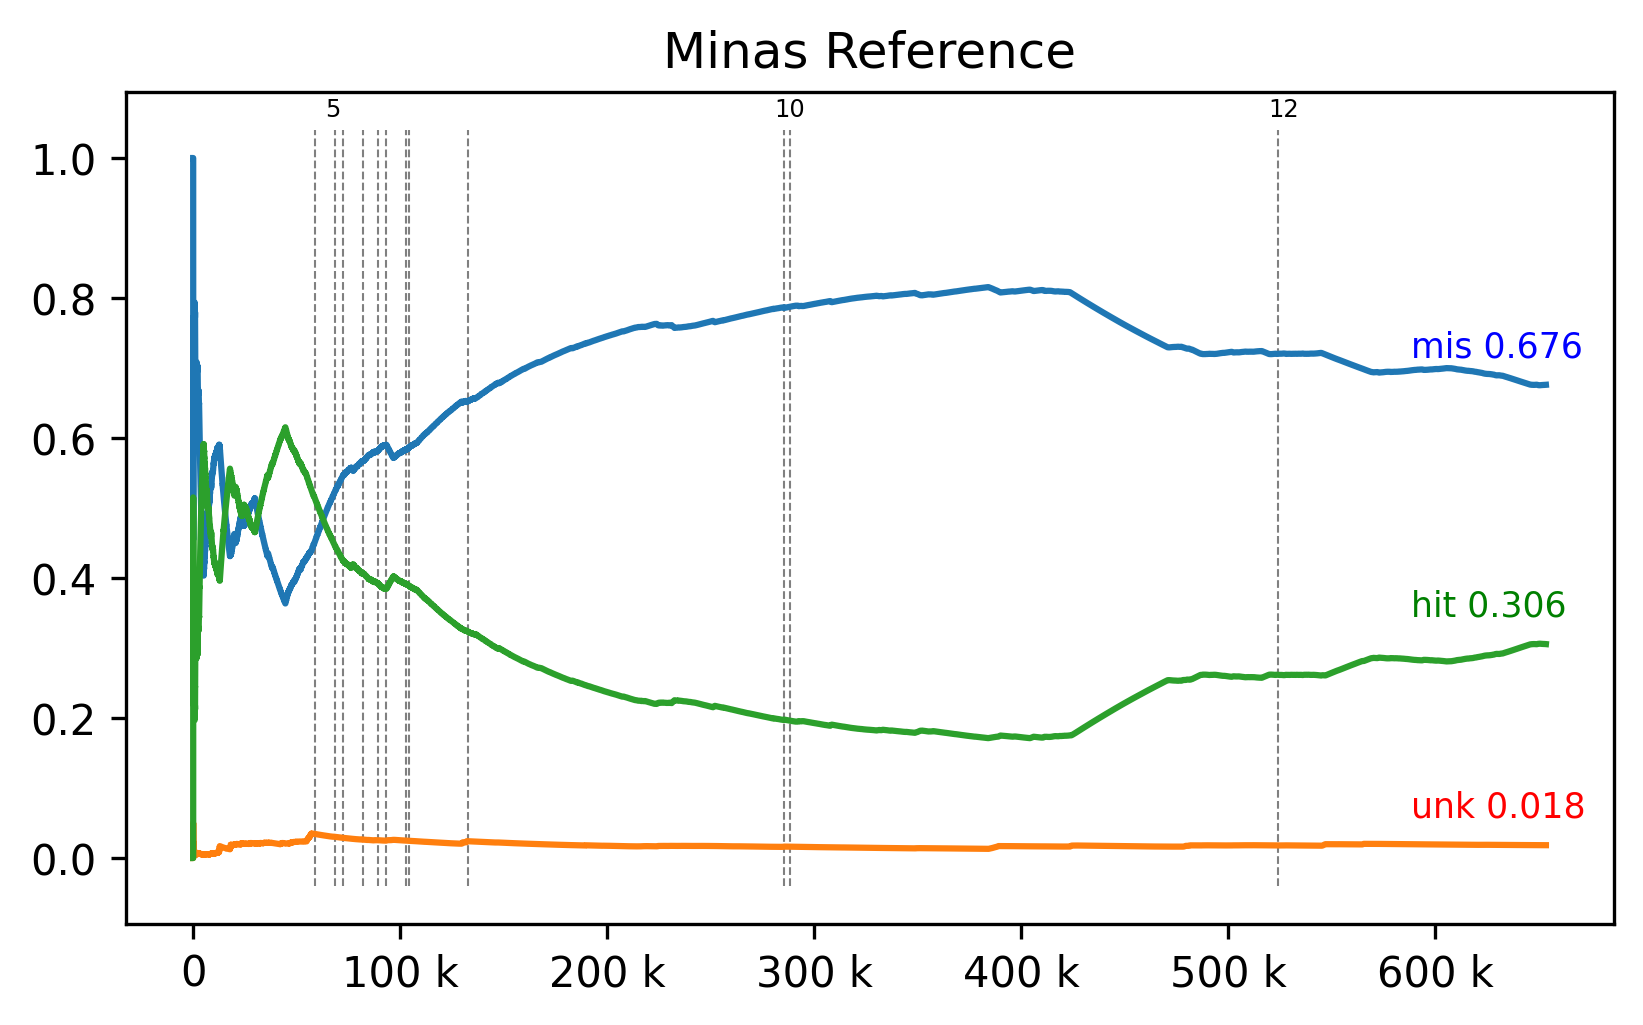
\includegraphics[width=\linewidth]{revised-java.log.png}
      \caption{Reference Implementation}
      \label{fig:validation-sub-java}
    \end{subfigure}
    \begin{subfigure}{.5\textwidth}
      \centering
      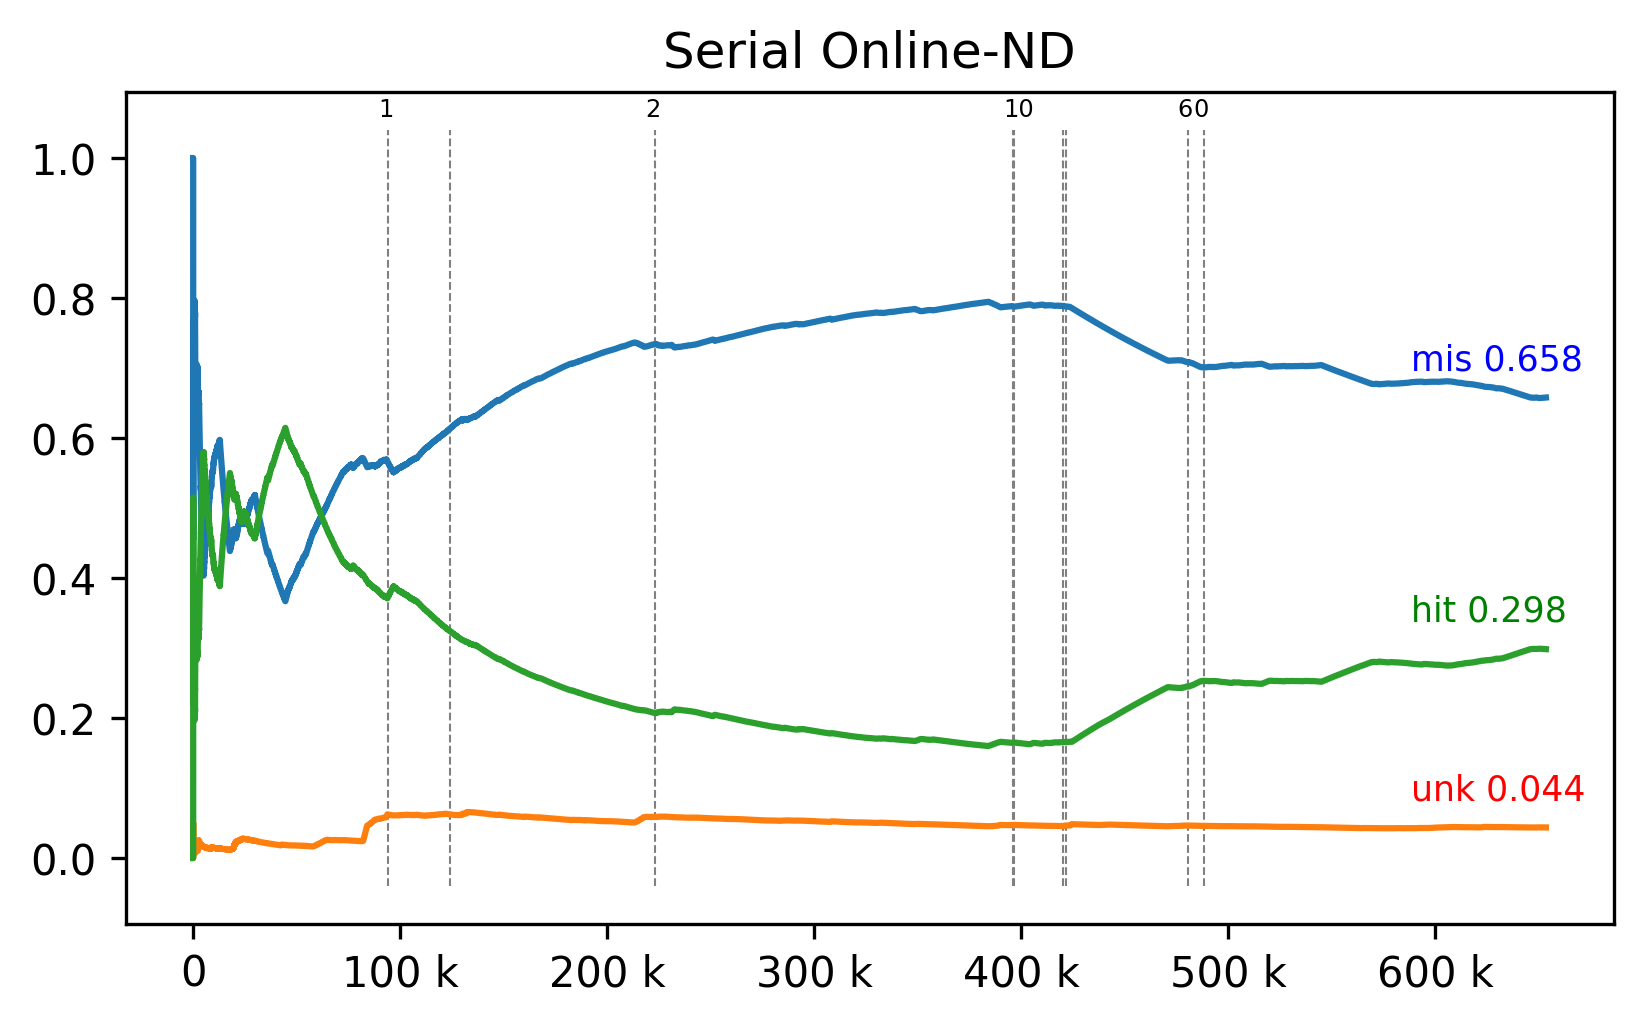
\includegraphics[width=\linewidth]{online-nd.log.png}
      \caption{Sequential Implementation}
      \label{fig:validation-sub-serial}
    \end{subfigure}
  }
  \centerline{
    \begin{subfigure}{.5\textwidth}
      \centering
      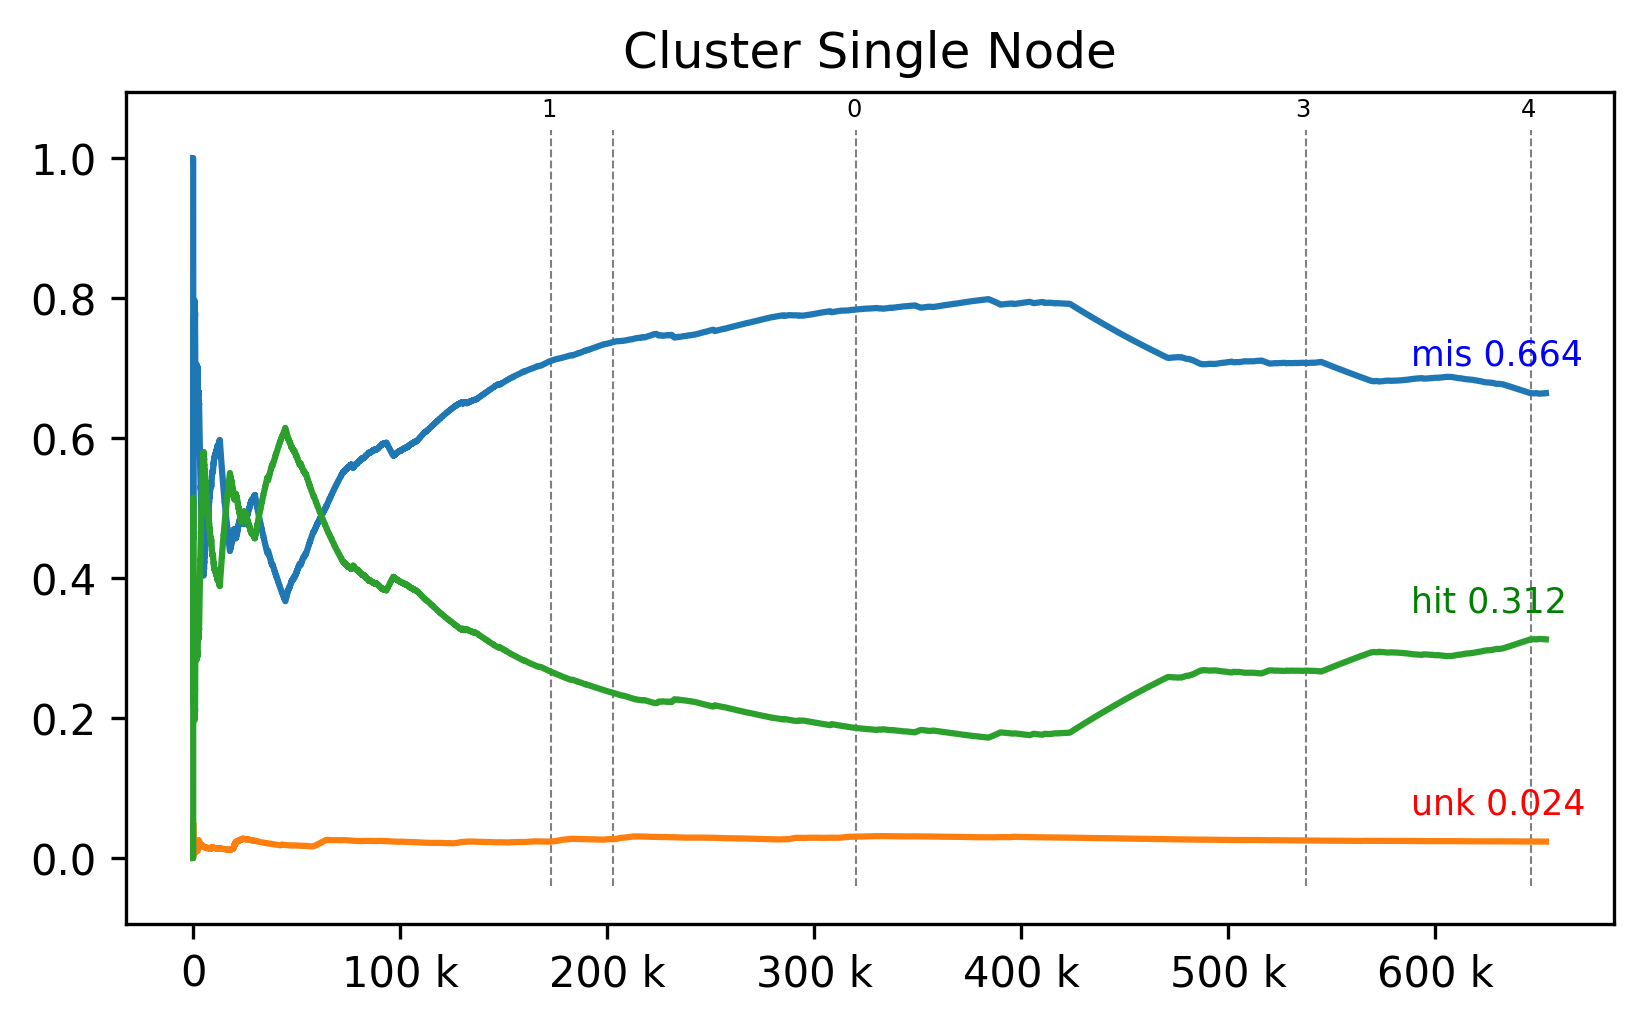
\includegraphics[width=\linewidth]{tmi-base.log.png}
      \caption{Parallel single-node}
      \label{fig:cluster-sub-single}
    \end{subfigure}
    \begin{subfigure}{.5\textwidth}
      \centering
      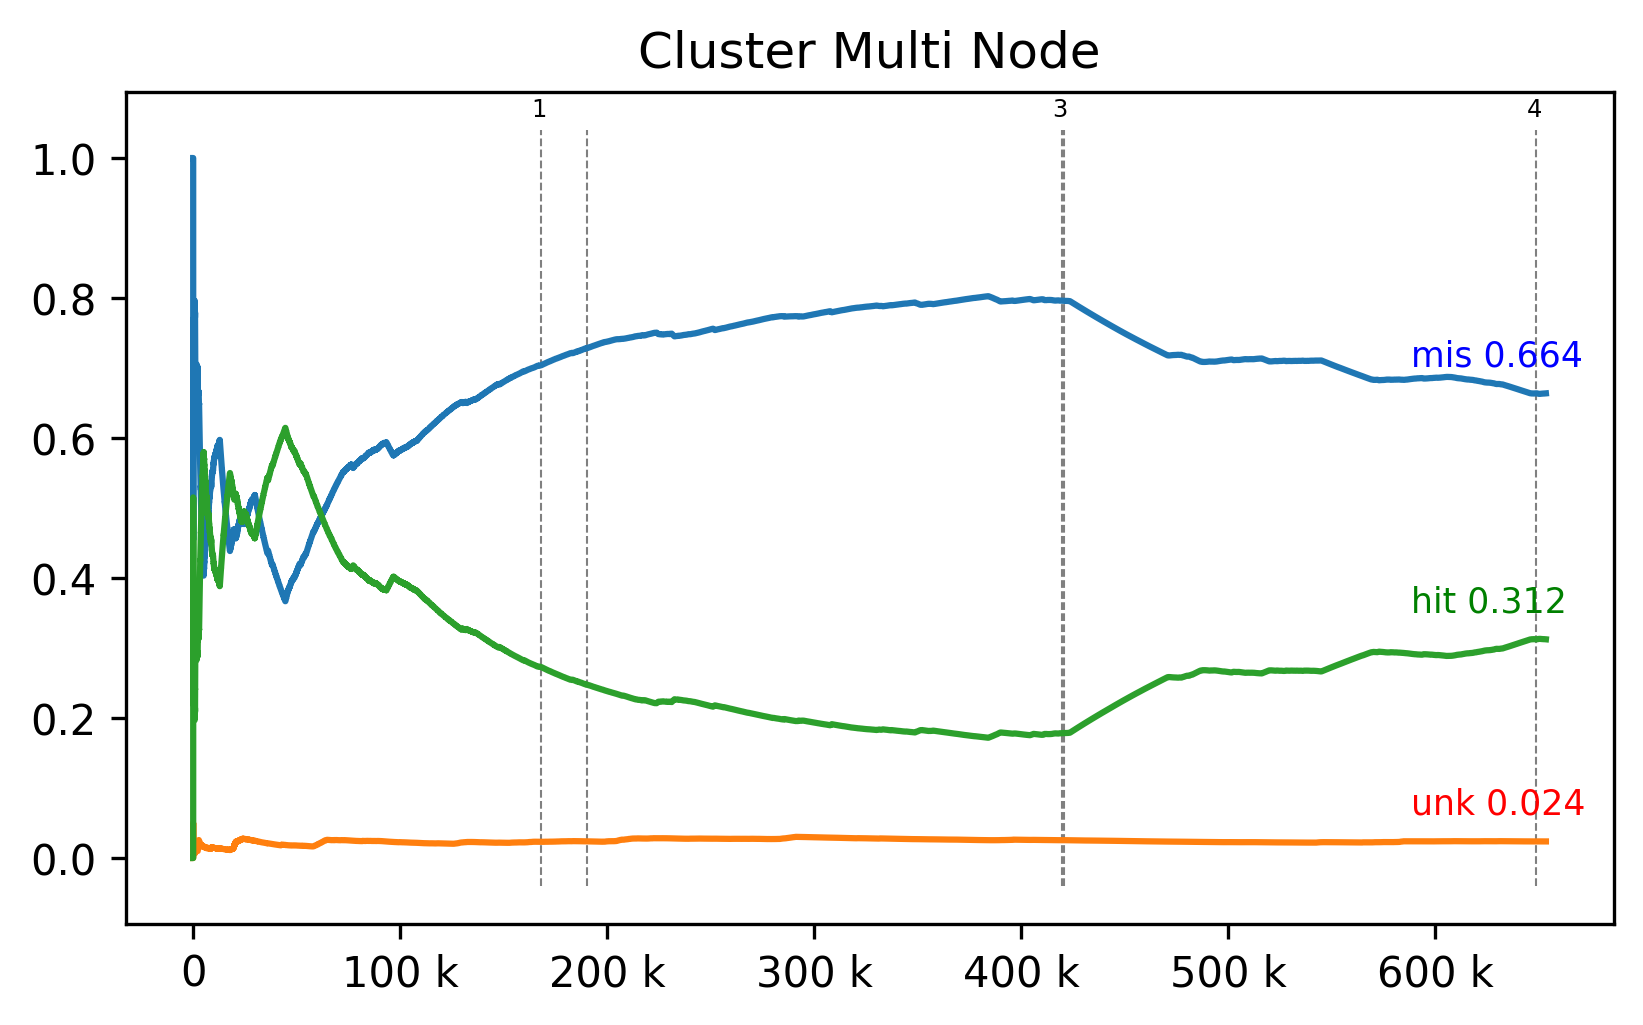
\includegraphics[width=\linewidth]{tmi-n12.log.png}
      \caption{Parallel multi-node}
      \label{fig:cluster-sub-multi}
    \end{subfigure}
  }
  % \caption{Validation Comparison: Stream hits and novelties visualization}
  % \label{fig:validation-java-serial}
  \caption{Stream hits and novelties visualization.}
  \label{fig:visualization}
\end{figure*}

% \hl{END Oritações de leitura das métricas e visualizações.}

% \FloatBarrier
\subsection{Discussion}

Four main experiments are presented for discussion:
(\emph{a}) reference implementation of \minas (\refminas) \cite{Faria2016minas};
(\emph{b}) new implementation in sequential mode;
(\emph{c}) new implementation in single-node, multi-process mode ($1\times4$) and
(\emph{d}) new implementation in multi-node, multi-process mode ($3\times4$).
Each experiment uses the adequate binary executable, initial model
(or training set for \refminas) and test set
to compute a resulting output stream which is stored for qualitative evaluation.
The summary of all four experiments is shown in Table \ref{tab:exper-summary}.

\begin{table*}[hbt]
\begin{center}
  \caption{Collected Measures Summary.}
  \label{tab:exper-summary}
  % % \begin{tabular}{l|r|r|r|r}
%          &    Exp. (a)  & Exp. (b)   & Exp. (c)    & Exp. (d)   \\\hline
% Hits     &     0.305618 &   0.298438 &    0.312416 &    0.312478    \\\hline
% Misses   &     0.676049 &   0.657843 &    0.664061 &    0.663802    \\\hline
% Unknowns &     0.018333 &   0.043717 &    0.023521 &    0.023718    \\\hline
% Time     &  2761.830000 &  80.790000 &  522.100000 &  207.140000    \\\hline
% System   &     7.150000 &  11.510000 &   47.770000 &  157.610000    \\\hline
% Elapsed  &  2772.070000 &  93.030000 &  145.040000 &   95.380000    
% \end{tabular}

% java -ea -classpath bin/minas/revised.jar: NoveltyDetection.MinasRevised datasets/training.csv datasets/test.csv out/revised-java.log true
% 	2761.82 user	7.15 system	46:12.07 elapsed

% ./bin/offline
% 	193.94 user	0.05 system	3:14.04 elapsed

% "./bin/ond
% 	80.79 user	11.51 system	1:33.02 elapsed

% mpirun -n 12 -hostfile ./conf/hostsfile ./bin/tmpi
% 	207.13 user	157.61 system	1:35.38 elapsed

\newcommand{\mr}[1]{\multirow{2}{*}{#1}}

\begin{tabular}{l|r|r|r|r|r}
                & \refminas (a)  & Offline       & Serial (b)      & Single Node (c) & Multi Node (d)  \\\hline
\mr{Hits}       & $\ 199708\ $   &               & $\ 195017\ $    & $\ 204151\ $    & $\ 204191\ $    \\
                & $\ 0.305618\ $ &               & $\ 0.298438\ $  & $\ 0.312416\ $  & $\ 0.312478\ $  \\
\hline
\mr{Misses}     & $\ 441769\ $   &               & $\ 429873\ $    & $\ 433936\ $    & $\ 433767\ $    \\
                & $\ 0.676049\ $ &               & $\ 0.657843\ $  & $\ 0.664061\ $  & $\ 0.663802\ $  \\
\hline
\mr{Unknowns}   & $\ 11980\ $    &               & $\ 28567\ $     & $\ 15370\ $     & $\ 15499\ $     \\
                & $\ 0.018333\ $ &               & $\ 0.043717\ $  & $\ 0.023521\ $  & $\ 0.023718\ $  \\
\hline
Time            & $\ 2761.83\ $  & $\ 194.12\ $  & $\ 80.79000\ $  & $\ 522.1000\ $  & $\ 207.1400\ $  \\\hline
System          & $\ 7.15\ $     & $\  0.075\ $  & $\ 11.51000\ $  & $\  47.7700\ $  & $\ 157.6100\ $  \\\hline
Elapsed         & $\ 2772.07\ $  & $\ 194.27\ $  & $\ 93.03000\ $  & $\ 145.0400\ $  & $\  95.3800\ $  
\end{tabular}


  \newcommand{\mr}[1]{\multirow{2}{*}{#1}}
  \setlength\extrarowheight{2pt}
  \begin{tabular}{l|r|r|r|r|r}
    % Experiment      & \expA         & \emph{Offline} & \expB     & \expC    & \expD    \\
    Experiment      & \refminas (a) & Offline       & Sequential (b)  & Single Node (c) & Multi Node (d)  \\
    Metric          &               &               &                 &                 &        \\\hline
    \mr{unk}        & $11980$       &               & $28567$         & $15370$         & $15499$     \\
                    & $0.018333$    &               & $0.043717$      & $0.023521$      & $0.023718$  \\\hline
    \mr{hit}        & $199708$      &               & $195017$        & $204151$        & $204191$    \\
                    & $0.305618$    &               & $0.298438$      & $0.312416$      & $0.312478$  \\\hline
    \mr{err}        & $441769$      &               & $429873$        & $433936$        & $433767$    \\
                    & $0.676049$    &               & $0.657843$      & $0.664061$      & $0.663802$  \\\hline
    Time      ($s$) & $2761.83$     & $194.12$      & $80.79$         & $522.10$        & $207.14$    \\\hline
    System    ($s$) & $7.15$        & $ 0.075$      & $11.51$         & $ 47.77$        & $157.61$    \\\hline
    Elapsed   ($s$) & $2772.07$     & $194.27$      & $93.03$         & $145.04$        & $ 95.38$    \\\hline
    Latency   ($s$) & $4.24\cdot10^{-3}$  &         & $1.42\cdot10^{-4}$  & $2.22\cdot10^{-4}$  & $1.46\cdot10^{-4}\ $  \\\hline
    Processors      & $1$           &  $1$          &  $1$            & $4$         & $12$        \\\hline
    Speedup         &               &               &                 & $0.6414092$ & $0.9753617$  \\\hline
    Efficiency      &               &               &                 & $0.1603523$ & $0.0812801$  
  \end{tabular}
\end{center}
\end{table*}

The comparison of the first two experiments (\emph{a} and \emph{b}) provides a
validation for our implementation, while the latter three (\emph{b}, \emph{c}
and \emph{d}) serve as showcase for the effects of distribution.

As stated, to validate our implementation we have compared it to \refminas
(the original \minas companion implementation), so we extracted the same measurements
using same process for both \emph{a} and \emph{b}, which can be viewed in
Tables \ref{tab:java-matrix}, \ref{tab:libc-matrix} and for ease of comparison
in Table \ref{tab:exper-summary} the summary can be compared side by side.

In general, the observed classification quality measurements are very similar,
and only diverge slightly where \emph{a} has more \emph{Hits} and \emph{Misses}
whereas \emph{b} shifted those to \emph{Unknowns}.
This phenomenon was watched very closely during development and we found that it was due to
small changes to \minas parameters, \minas internals like K-means ordering,
cluster edge inclusion and cluster radius formula as stated in
Subsection \ref{sec:implementation}.

As for the time measurements in Table \ref{tab:exper-summary}
our implementation used less time to analyze the test data set.
This is mostly due to 
the stop condition
on the internal K-means algorithm; while \refminas uses a fixed iteration
limit of $100$, our implementations adds the ``no improvement'' check
and stops earlier in most cases, which in turn reduces the time taken
on the \emph{NoveltyDetection} function.
There are also small optimizations on the \emph{nearestCluster} function
(minimal distance from sample to cluster center in the set)
affecting the \emph{classifier} task and \emph{NoveltyDetection} function.
One can also note that \refminas time in \emph{a} includes the Offline phase while our
implementation runs it once and reuses the initial model for \emph{b}, \emph{c}
and \emph{d}. In the table the offline time this is shown as a separate column.

As for the effects of running the classification processes on the small devices as MPI nodes with our implementation, we observe
an increase of time when we go from $1$ to $4$ instances in a single node
(\emph{b} and \emph{c} respectively), hinting that our choice of load
distribution is not as effective as we expected.
Further experiments were conducted with the number of instances varying from $1$ (sequential) to
$12$ (3 nodes with 4 CPUs each), but that caused no impact on the true positive rate (\emph{Hits}) and elapsed time.
More detailed time measurements can be seen in Figure \ref{fig:speedup},
where we observe near constant time for \emph{elapsed} (near $100s$),
the \emph{system} increases gradually while \emph{user} decreases at the same rate.
We interpret this behavior as a display of potential for gains using a better
load balancing than our choice of round-robin such as micro-batching for better
\emph{compute-to-communication ratio} (CCR).
% legal!
In general, Figure \ref{fig:speedup} shows no speedup but also no penalty for
scaling to more than $4$ instances.

% \st{we have to say it is pretty shitty because of our choice of distribution 
% using round-robin, use some load balancing and micro-batching for better results.}

% Tempo gasto com distribuição e tempo gasto com processamento mostra que é viável.

% relação $p/n$ 

% relação do tempo comm / tempo processing
% coom time / processing time does not inhibit the use of our aproach.
% CCR

% compute-to-communication ratio (CCR) indicates that our approach is viable 

% compute-to-communication ratio (CCR).

\begin{figure}[hbt]
  \centering
  % 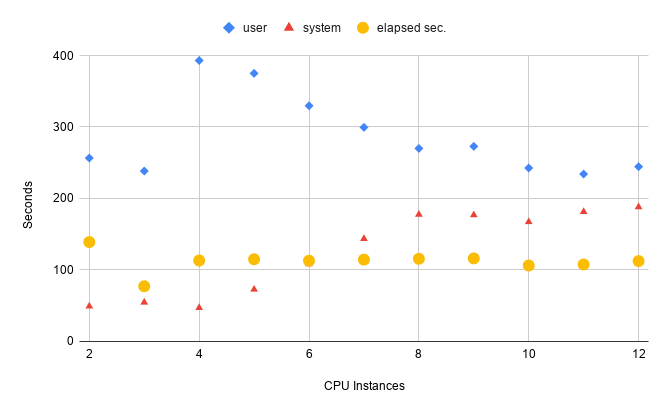
\includegraphics[width=\linewidth]{experiments/speedup-clean.png}
  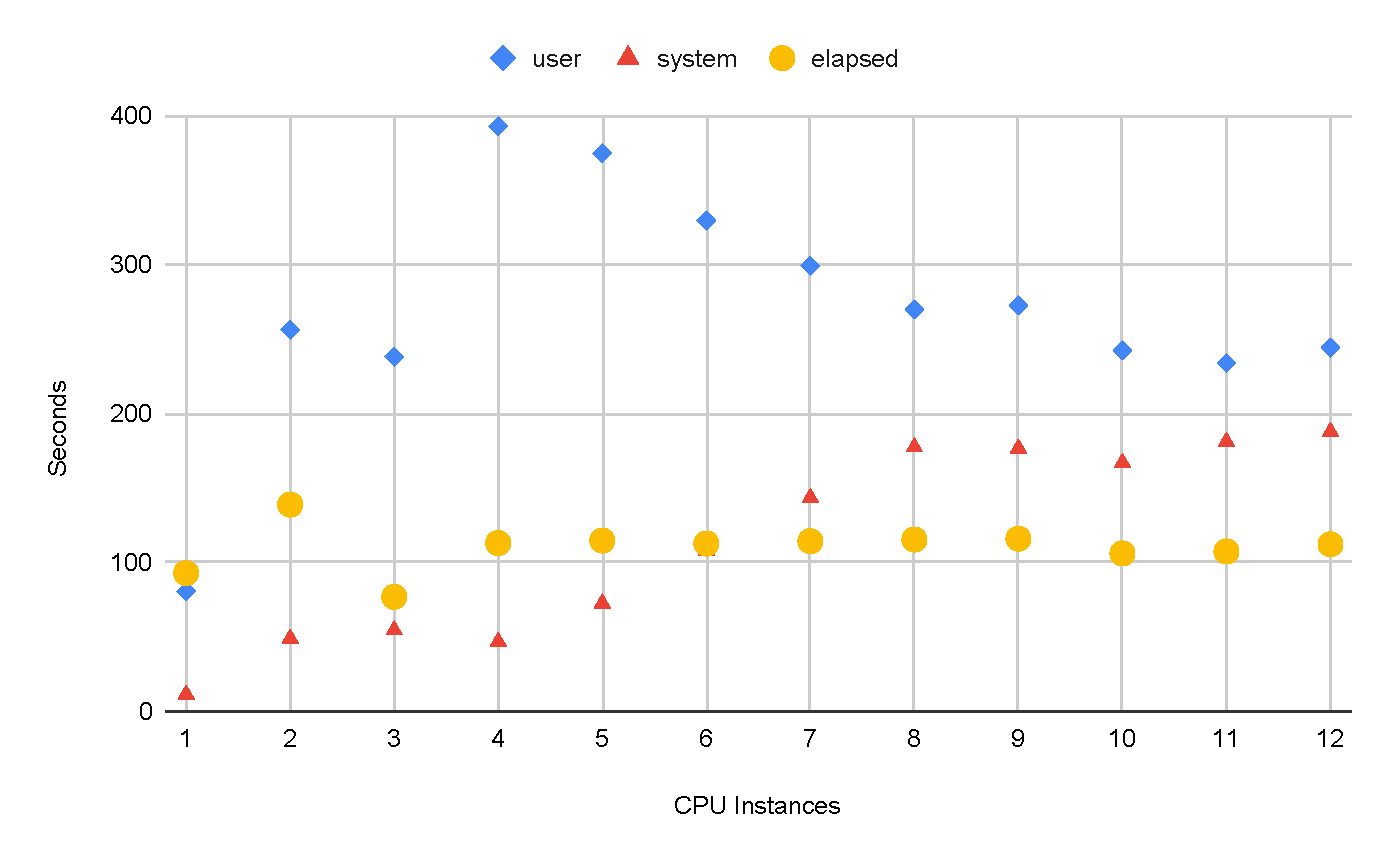
\includegraphics[width=1\linewidth,page=1]{speedup-clean.pdf}
  \caption{Time measurements per added instance.}
  \label{fig:speedup}
\end{figure}

Nevertheless, we can also show the effects of delay in the
Classify, Novelty Detection, Model Update and Classify feedback loop.
Comparing \emph{b} and \emph{c} we observe a reduction in Novelty labels
on the Confusion Matrix (tabs. \ref{tab:libc-matrix} and \ref{tab:single-node-matrix})
from $9$ to $5$.
The same effect is observed on the stream visualization (figs.
\ref{fig:validation-sub-serial} and \ref{fig:cluster-sub-single}) where our
sequential implementation has fewer novelty markers, and they appear later, but the
measures keep the same ``shape''.
Comparing \emph{c} and \emph{d} the difference is even smaller,
(figs. \ref{fig:validation-sub-serial} and \ref{fig:cluster-sub-single})
as they both suffer the expected delay in the feedback loop due to asynchronous
task execution.
